\documentclass[11pt,a4paper]{moderncv}
\moderncvtheme[blue]{classic}                
\usepackage[utf8]{inputenc}
\usepackage[top=0.9cm, bottom=0.9cm, left=1.4cm, right=1.4cm]{geometry}
\usepackage[english]{babel}
\setlength{\hintscolumnwidth}{2.9cm} % width of the left column (dates)
%\setlength{\makecvtitlenamewidth}{20cm}

\firstname{Romain}
\familyname{Pellerin}
\title{Software Engineering Student}
%\photo[64pt][0.0pt]{picture} % '64pt' is the height the picture must be resized to, 0.0pt is the thickness of the frame around it (put it to 0pt for no frame) and 'picture' is the name of the picture file       
\address{}{Paris, Fance}{} % street, city, country
\email{contact@romainpellerin.eu}                      
\homepage{romainpellerin.eu}
\mobile{+33-7 85 25 71 64} 
\extrainfo{\href{https://github.com/rpellerin}{github.com/rpellerin}}
\quote{Objective: a 6-month internship in software development starting from September 2015}
\renewcommand*{\quotefont}{\Large\bfseries} % override quote's default style

% I took the original code from moderncvstylebanking.sty and changed line 25
% USEFUL for theme banking
% \makeatletter
% \renewcommand*{\maketitle}{%
%   \setlength{\maketitlewidth}{1.0\textwidth}%
%   \hfil%
%   \parbox{\maketitlewidth}{%
%     \centering%
%     % name and title
%     \namestyle{\@firstname~\@lastname}%
%     \ifthenelse{\equal{\@title}{}}{}{\titlestyle{~|~\@title}}\\% \isundefined doesn't work on \@title, as LaTeX itself defines \@title (before it possibly gets redefined by \title) 
%     % detailed information
%     \addressfont\color{color2}%
%     \ifthenelse{\isundefined{\@addressstreet}}{}{\addtomaketitle{\addresssymbol\@addressstreet}%
%       \ifthenelse{\equal{\@addresscity}{}}{}{\addtomaketitle[~--~]{\@addresscity}}% if \addresstreet is defined, \addresscity and \addresscountry will always be defined but could be empty
%       \ifthenelse{\equal{\@addresscountry}{}}{}{\addtomaketitle[~--~]{\@addresscountry}}%
%       \flushmaketitle\@firstmaketitleelementtrue\\}%
%     \collectionloop{phones}{% the key holds the phone type (=symbol command prefix), the item holds the number
%       \addtomaketitle{\csname\collectionloopkey phonesymbol\endcsname\collectionloopitem}}%
%     \ifthenelse{\isundefined{\@email}}{}{\addtomaketitle{\emailsymbol\emaillink{\@email}}}%
%     \ifthenelse{\isundefined{\@homepage}}{}{\addtomaketitle{\homepagesymbol\httplink{\@homepage}}}%
%     \collectionloop{socials}{% the key holds the social type (=symbol command prefix), the item holds the link
%       \addtomaketitle{\csname\collectionloopkey socialsymbol\endcsname\collectionloopitem}}%
%     \ifthenelse{\isundefined{\@extrainfo}}{}{\addtomaketitle{\@extrainfo}}%
%     \flushmaketitle}\\[2.5em]}% need to force a \par after this to avoid weird spacing bug at the first section if no blank line is left after \maketitle
%  \makeatother

\begin{document}
\makecvtitle

\section{Professional Experience}
\cventry{September 2014 -- present}{Computer Science Manager}{\href{http://www.usec-utc.fr/}{USEC}}{Compiègne (France)}{}{I'm in charge of software development projects for local companies.
\begin{itemize}
  \item Writing official documents (quotes, specifications, customer agreements, etc.)
  \item Recruiting and mentoring students (those who develop our clients' projects)
\end{itemize}}
\cventry{June 2013 -- September 2014}{Android and web developer}{Self-employed (\textit{Auto-entrepreneur})}{Nantes (France)}{}{Developed and then updated the Android application and the website of the startup \textsc{\href{http://www.who-wanna.com/en/}{WhoWanna}}.}%\newline{}

\cventry{April 2014 -- June 2014}{Intern in software development}{\href{http://www.who-wanna.com/en/}{WhoWanna}}{Nantes (France)}{}{
\begin{itemize}%
\item Migrated data onto a "cloud" solution (\href{http://www.clever-cloud.com/}{Clever Cloud})
\item Updated the Android application (added some features, graphical update)
\item Started to change the language and the DBMS used on the server: from PHP to Scala and from MySQL to PostgreSQL
\item Wrote internal documentation (\LaTeX{} and a website) and set up a versioning system (Git)
\end{itemize}}

\section{Volunteer Experience}
\cventry{2015 -- present}{President and co-organizer of tech talks}{\href{https://www.youtube.com/playlist?list=PL3nMxbEwNq0wE3BNx5b0EEtp8h-yvHyIy}{HumanTalks}}{Compiègne (France)}{}{10-minute talks given once a month about programming languages, tools, software development, etc\\\href{http://humantalks.com/cities/compiegne}{http://humantalks.com/cities/compiegne}}

\section{Education}
\cventry{2014 -- present}{Software Engineering}{\href{http://www.utc.fr/formations-enseignements/genie-informatique.php}{Université de Technologie de Compiègne}}{Compiègne (France)}{Expected June 2017}{} % year, degree, institution, city+picture = {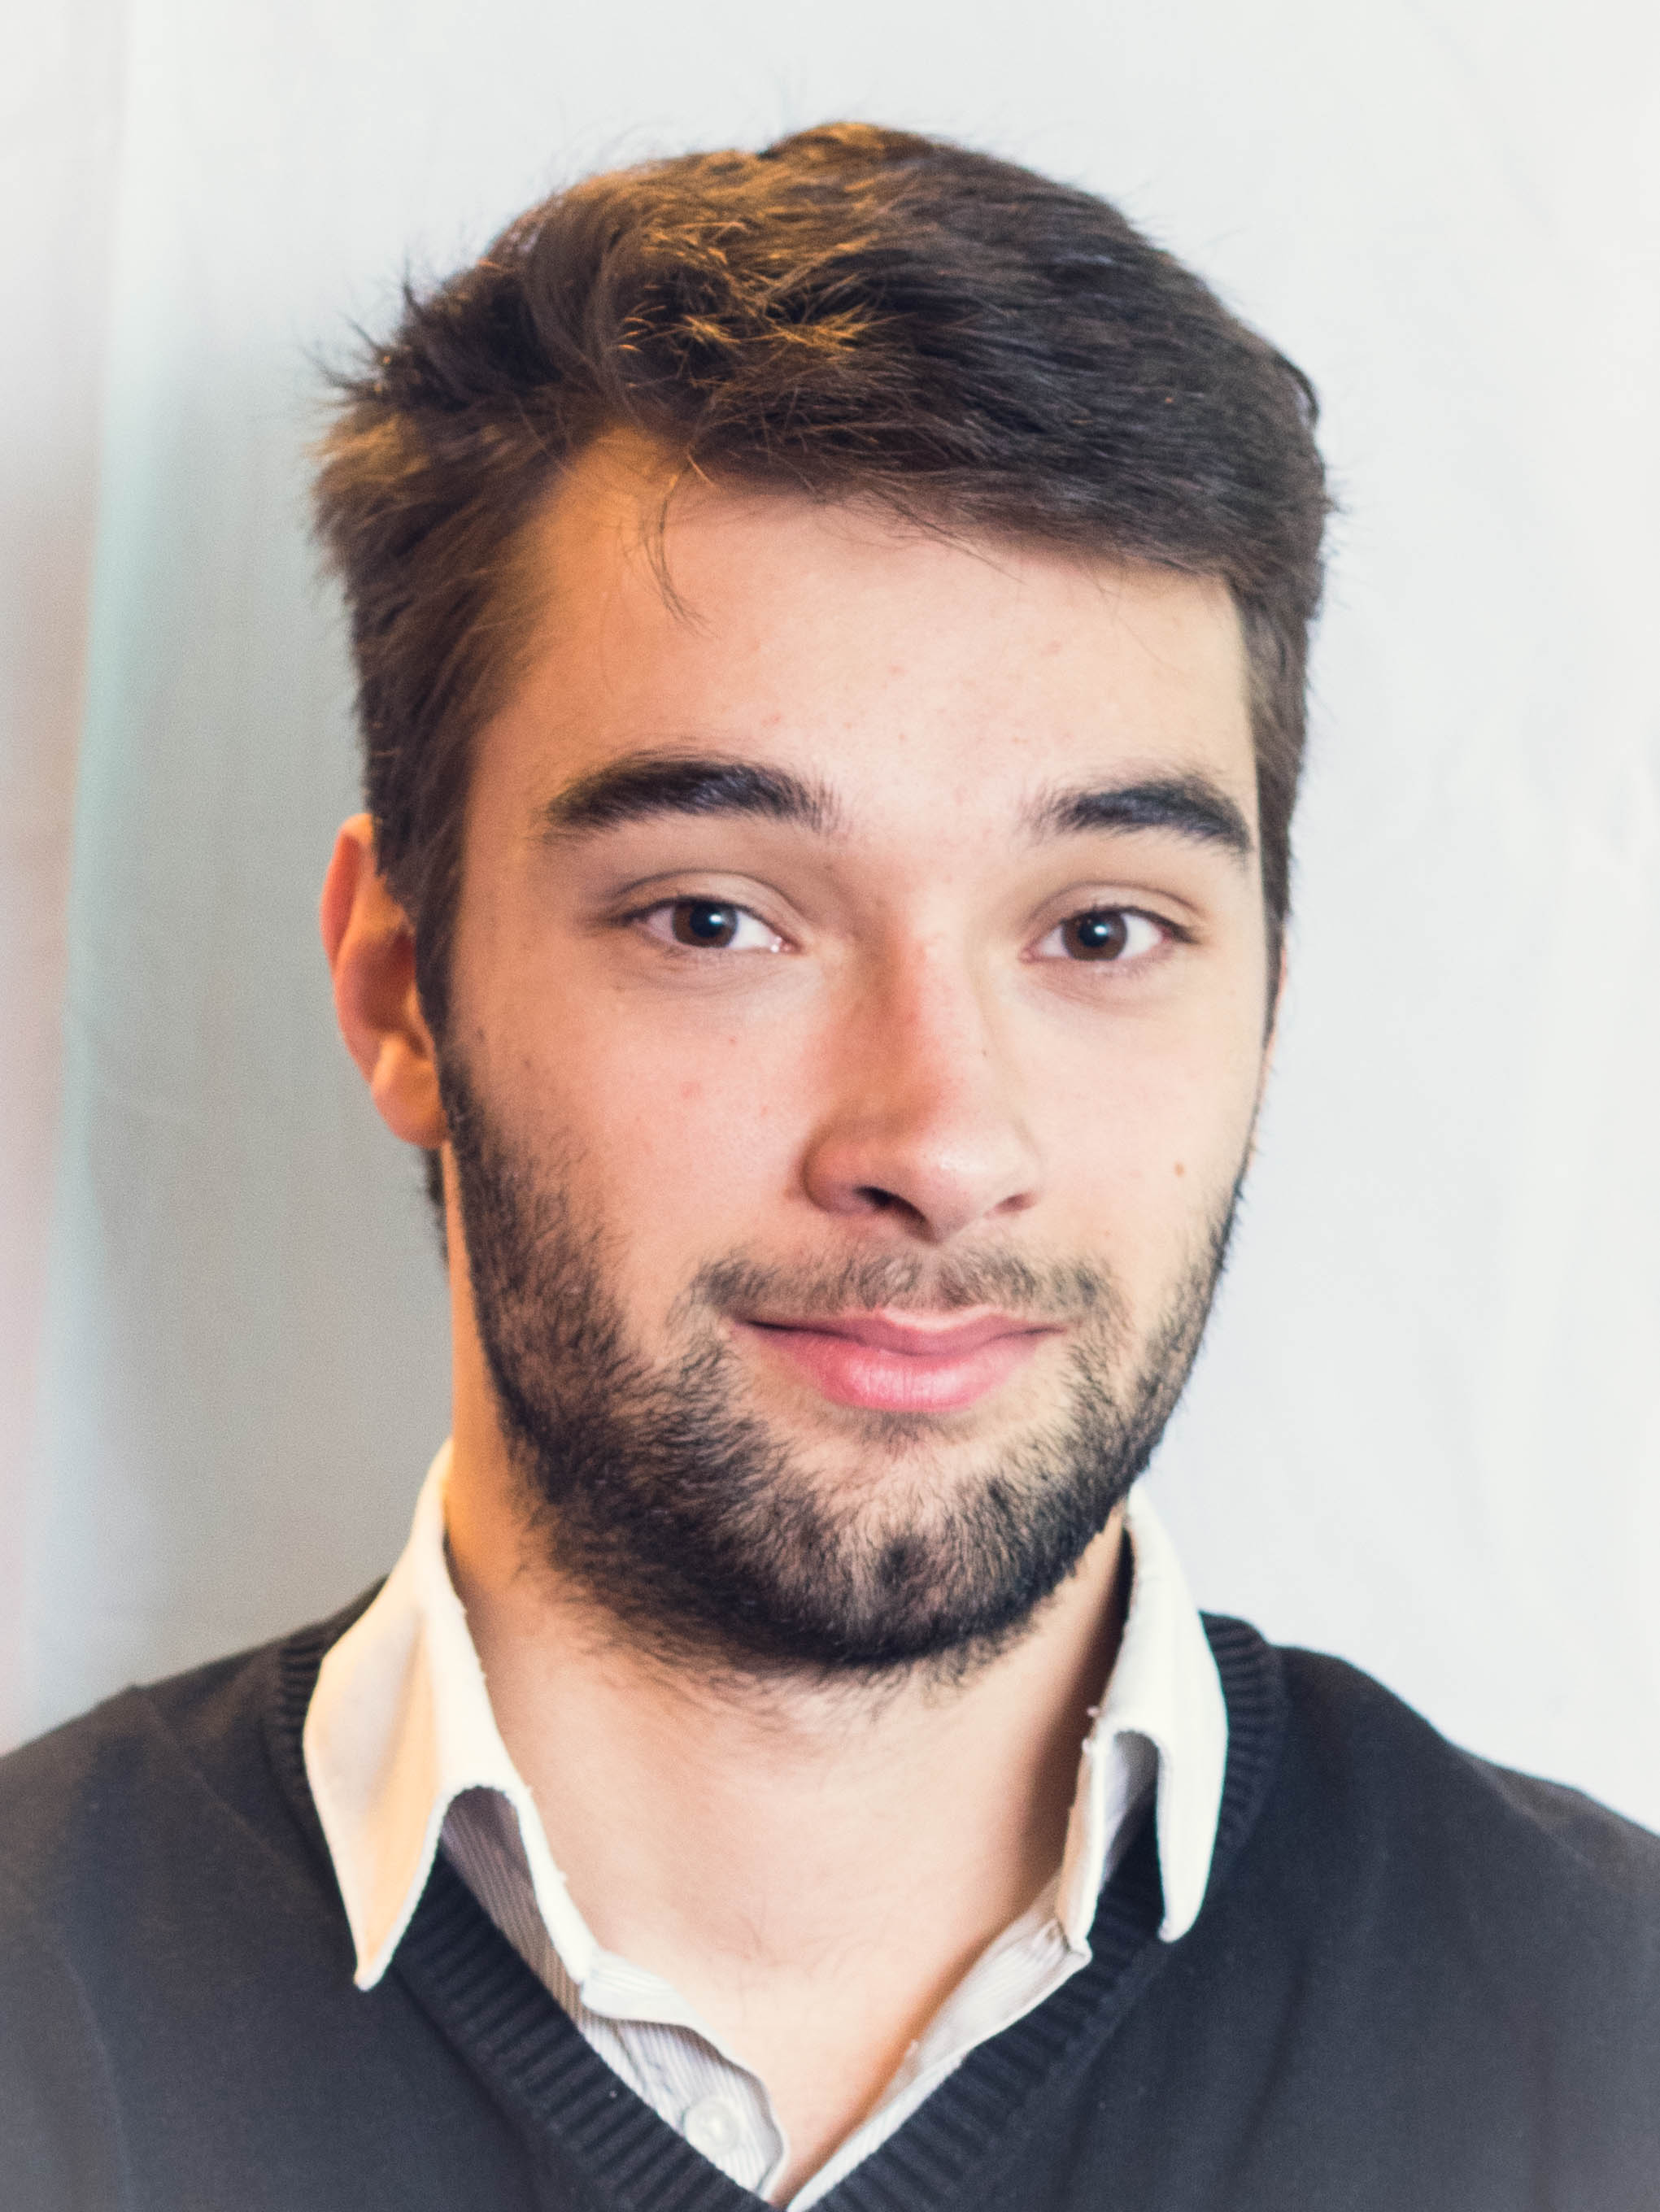
\includegraphics[scale=0.5]{picture}City}, grade, description
\cventry{2012 -- 2014}{Two-year core studies diploma in Computer Science (DUT Informatique)}{\href{http://www.iutnantes.univ-nantes.fr/321/0/fiche___formation/}{Nantes University Institute of Technology (IUT de Nantes)}}{Nantes (France)}{}{}

\section{Computer Skills}
% \cvcomputer{category}{programs}{category}{programs}
% \cvdoubleitem{subtitle}{text}{subtitle}{text}
\cvitem{Languages}{\textbf{C, C++ (Qt), Java (SE \& EE), PHP, HTML, CSS}, JavaScript, Bash, x86 assembly}
\cvitem{Modeling}{\textbf{UML}}
\cvitem{Databases}{\textbf{MySQL, PostgreSQL}}
\cvitem{OSs}{\textbf{GNU/Linux (Debian)}, Windows XP/7/8}
\cvitem{Other}{\textbf{Git, Apache2}, iptables, fail2ban, OpenVPN, Subversion, TCP/IP, \LaTeX}

\section{Languages}
\cvlanguage{French}{Native speaker}{}
\cvlanguage{English}{Fluent (European B2 level)}{\textbf{Toeic 895/990}}

\section{Hobbies}
\cvdoubleitem{Conferences}{\href{http://devfest.gdgnantes.com/}{DevFest} (Nantes, France), \href{http://web2day.co/}{Web2Day} (Nantes, France)}{Free software}{Fervent defender, I always push my source code on \href{https://github.com/rpellerin}{GitHub}}
\cvdoubleitem{\textbf{Raspberry Pi}}{\textbf{Self-hosted websites, VPN, ownCloud, proxy}}{\textbf{Many side-projects}}{\textbf{Android applications, web browser add-ons, websites}}
\cvdoubleitem{Music}{I have been playing the guitar for nine years}{Sport}{Workout, badminton}
\end{document}
